Di seguito viene spiegato l'utilizzo delle principali funzioni dell'applicazione
\section{Registrazione}
Per creare un nuovo account selezionare il tasto \textbf{Sign Up} posizionato in alto a destra dello schermo.

\noindent Ora bisogna compilare un piccolo form che richiede alcuni dati necessari per poter effettuare la registrazione: username, email, first name, last name, password e verifica password.

\noindent Una volta compilati tutti i campi richiesti premere il bottone \textbf{Sign Up} situato sotto il form.

\section{Autenticazione}
Se si possiede già un account è possibile effettuare l'autenticazione.

\noindent Per autenticarsi premere il pulsante \textbf{Login} situato in alto a destra dello schermo accanto al pulsante di registrazione.

\noindent Ora sono richiesti i dati d'accesso.

\begin{figure}[h] 
	\centering 
	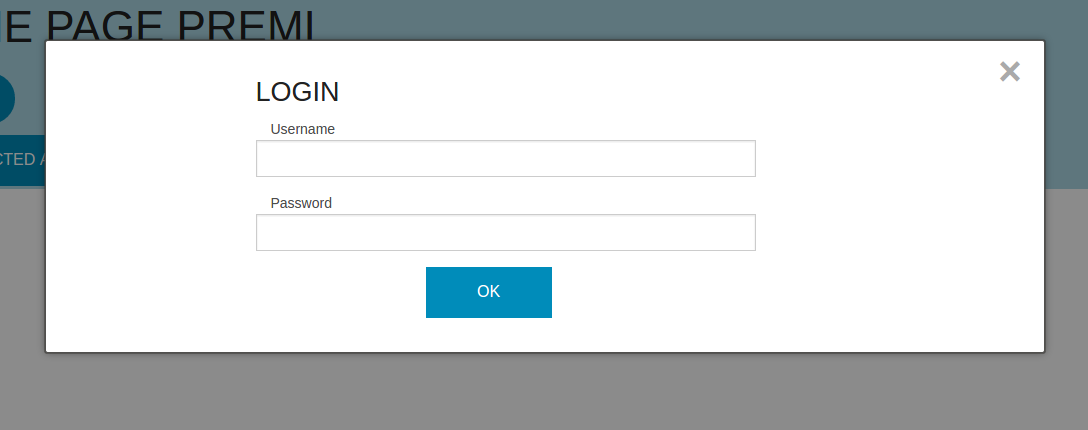
\includegraphics[scale=0.40] {img/MULogin.png}
	\caption{UC1 - Registrazione} 
\end{figure}

\noindent Una volta inseriti premere il pulsante \textbf{Login} situato sotto il form.

\section{Creazione di un Progetto}

Effettuata l'autenticazione è possibile cominciare a creare progetti.


\noindent Per creare un progetto selezionare dal menù in alto \textbf{New Project} e inserite un titolo per il progetto.


\section{Creazione di una Presentazione}

Una volta creato un progetto verrà automaticamente aperto l'editor che permette di creare le slide della presentazione.

\section{Creazione di un'Infografica}

Per creare un'infografica è sufficiente aprire un progetto e premere il pulsante \textbf{New Infographic}; dal menù laterale e verrà aperto l'editor con cui è possibile modificare l'infografica.

\section{Ricerca di un progetto}

È possibile fare una ricerca tra i progetti salvati da altri utenti.

\noindent Per fare ciò è sufficiente compilare il filtro di ricerca, presente sulla propria home page, e premere il pulsante \textbf{Search}.

Verrà visualizzata una lista di progetti che rispettano i parametri inseriti.

\noindent A questo punto basta selezionarne uno e scegliere la modalità di visualizzazione.